Figure \ref{fig:results} shows charge to discharge ratio from the practical system. As compared to the theoretical result shown in figure \ref{fig:crs} (a) a clear degradation can be noticed. The average value has been reduced from 6 to 4.75. This is due to two major reasons, the imperfection of practical components and the assumptions taken in the theoretical model. In theoretical model we made the assumption that during the charge cycle there is no current flowing into the battery and $i_r \approx i_c $, where as in reality a small current is flowing into the battery hence producing the non ideality in the actual results.
  
%---------- Charge to Discharge ratio from the actual circuit
%
\begin{figure}[h!]
\centering
\includegraphics[width=0.8\textwidth]{results.pdf}
\caption{Charge to discharge Ratio}
\label{fig:results}
\end{figure}
%


%-----------------------Table ----------------------------------------
\begin{tabular*}{\textwidth}{@{\extracolsep{\fill}} |l|l|}
\hline
Distance between two coils (cm) & Efficiency (\%) \\
\hline
0 & 70 \\
\hline
1 & 40 \\
\hline
2 & 14.4 \\
\hline
3 & 8.2 \\
\hline
4 & 1.8 \\
\hline
\end{tabular*}
\begin{center}
\textbf{ Table 2.} Distance vs Efficiency
\end{center}

%---------- The dimension figure goes here

\begin{figure}[h!]
\centering
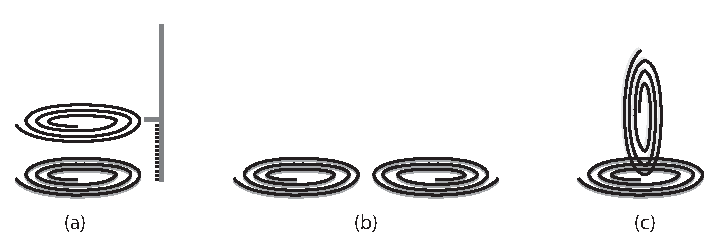
\includegraphics[width=0.9\textwidth]{dimension.pdf}
\caption{Orientations of the test set-up}
\label{fig:dimension}
\end{figure}


Table 2 shows the effect of distance on efficiency. It is clear from the table that an increase in distance between the two coils results in efficiency decrease and maximum achievable efficiency is 70 \%.  The overall efficiency is also affected by the orientation in which the two coils are placed. Three commonly possible orientations are shown in the figure \ref{fig:dimension}. The table 2 is formed with respect to the orientation shown in the figure \ref{fig:dimension} (a) where as orientations in \ref{fig:dimension} (b) and \ref{fig:dimension} (c) results in very low magnetic coupling between the coils and have tremendously low efficiency about in the order of 20 \% as a maximum which also decreases very rapidly with the increase in distance.


